\documentclass[preprint,9pt]{sigplanconf}

\usepackage{graphicx,listings,fixltx2e,lambda,array,times,color,algpseudocode}
\usepackage{stmaryrd}
\usepackage[usenames,dvipsnames]{xcolor}

\definecolor{lightgray}{rgb}{0.96,0.96,0.96}

\lstset{ 
  language=Python,                % the language of the code
  linewidth=230pt, 
  xleftmargin=8pt,
  basicstyle=\footnotesize\ttfamily, % Standardschrift
  numbers=none,                   % where to put the line-numbers
  numberstyle=\footnotesize,          % the size of the fonts that are used for the line-numbers
  stepnumber=1,                   % the step between two line-numbers. If it's 1, each line 
                                  % will be numbered
  numbersep=5pt,                  % how far the line-numbers are from the code
  showspaces=false,               % show spaces adding particular underscores
  showstringspaces=false,         % underline spaces within strings
  showtabs=false,                 % show tabs within strings adding particular underscores
  frame=single,                   % adds a frame around the code
  tabsize=2,                      % sets default tabsize to 2 spaces
  captionpos=b,                   % sets the caption-position to bottom
  breaklines=true,                % sets automatic line breaking
  breakatwhitespace=false,        % sets if automatic breaks should only happen at whitespace
  %title=\lstname,                   % show the filename of files included with \lstinputlisting;
                                  % also try caption instead of title
  numberstyle=\tiny\color{gray},        % line number style
  keywordstyle=\color{blue},          % keyword style
  commentstyle=\color{dkgreen},       % comment style
  backgroundcolor=\color{lightgray}, 
  belowskip=-10pt, 
  aboveskip=6pt, 
}

\begin{document}

\conferenceinfo{PLDI '13}{16--21 June 2013, Seattle, WA.} 
\copyrightyear{2013} 
\copyrightdata{[to be supplied]} 

\titlebanner{}        % These are ignored unless
\preprintfooter{PLDI 2013}   % 'preprint' option specified.

\title{Automated Adaptive Tuning of High Level Numerical Code}

\authorinfo{Name Omitted For Review}
           {Affiliation Omitted For Review}
           {omitted@omitted.com}

% define some useful commands to use in language specification 
\newcommand{\MAP}{\impfnt{map}}
\newcommand{\REDUCE}{\impfnt{reduce}}
\newcommand{\SCAN}{\impfnt{scan}}
\newcommand{\ALLPAIRS}{\impfnt{allpairs}}
\newcommand{\concat}{\ensuremath{+\!\!\!\!+\,}}

\maketitle

\begin{abstract}
In an ideal world, programmers could write code in high level languages and get excellent performance that was portable across multiple target platforms, input data sets, and execution conditions.  In reality, however, in order to get good performance programmers often have to write code in low level efficiency languages such as C++.  For numerical programs, they additionally have to parallelize their programs, add hooks for auto-tuners to use in setting optimization parameters, and wait for lengthy offline autotuning searches to complete before they are left with a high performance binary.  Even then, the binary is not portable across any of the variables mentioned above.  Thus, the state of the art falls far short of the ideal and involves a large burden on the programmer.

We present a system for accelerating numerical Python programs that addresses all of these issues. Programmers write code using Parakeet, a NumPy-like DSL for numerical programming embedded in Python that includes familiar higher-order data parallel primitives (referred to as \emph{adverbs}) including $\MAP$, $\REDUCE$, and $\SCAN$.  Our system is a JIT compiler and runtime for Parakeet that supports automatically parallelizing adverbs on multicore CPUs.  In addition, we introduce a novel code transformation for tiling adverbs directly that leaves tile sizes unspecified until runtime when an efficient online search is performed across different cache tile size settings.  Every step of the search involves useful work, and so the cost of tuning is much lower than in the offline case.  Finally, since the search is conducted online, it is adaptive both to the input data set as well as current execution conditions.

We evaluate our system on a suite of benchmark programs written in Parakeet.  We achieve excellent performance even compared with auto-tuned C code.  In addition, we show that the cost of the online search is low and that it quickly converges to good parameter settings.  Finally, we exhibit portable performance across different target platforms, input data sets, and system loads.
\end{abstract}

%\category{CR-number}{subcategory}{third-level}

%\terms
%term1, term2

%\keywords
%Compilers, Auto-Tuning, Online Optimization, Memory hierarchy, Tiling, Blocking, Unrolling, Program transformation, Code generation

\section{Introduction}
\label{intro}
A wide range of professionals -- from fields as diverse as the natural sciences to finance -- depend on numerical computing as an integral tool in their daily work that allows them to process massive data sets (so-called ``big data'').  These users often either (1) aren't expert programmers; or (2) don't have time to tune their software for performance, as their main job focus is not programming.  Thus these users typically prefer to use productivity languages such as Python or Matlab over efficiency languages such as C++ since productivity languages are much higher level and easier to use than efficiency languages~\cite{Pre03}.

However, such users do care about performance, especially since any inefficiencies in their code are magnified immensely by their data sets' large sizes.  Poorly tuned code can result in order of magnitude increases in runtimes, going from hours to days or days to weeks in some cases (INSERT REF).

We present a system that brings competitive and portable performance to a productivity language usable by numerical programmers.  Users write code in Parakeet~\cite{Rubi12}, a NumPy-like~\cite{Dubo96} DSL for numerical computing embedded in Python that includes familiar higher-order data parallel primitives (referred to as \emph{adverbs}) such as $\MAP$, $\REDUCE$, and $\SCAN$.  One can view Parakeet as a well-defined subset of NumPy plus adverbs, and users of the highly successful NumPy should feel right at home with Parakeet. Our system is a JIT compiler and runtime for Parakeet that targets multicore CPUs and includes support for automatic parallelization and online autotuning for performance.

A host of optimization strategies exist for tuning numerical programs, including cache tiling, register tiling, and loop unrolling~\cite{Chen05b, Cole95, Lam91, Wolf91}, and these optimizations are key to obtaining top performance~\cite{Frig05, Whal00, Yoto05}.  Unfortunately, these optimizations require setting parameters such as tile sizes and loop unrolling factors whose values depend on architectural details that are difficult to model.  Much work has gone into developing models in an attempt to enable performing these optimizations statically at compile time~\cite{Shir12, Yoto03, Yoto05}.

However, the state of the art for achieving top performance remains offline autotuning of programs to find good settings for these parameters~\cite{Asan06}.  Offline autotuning searches across different settings of parameters by timing the execution of different versions of the program on real hardware.  This approach burdens programmers in at least one of two ways: (1) it requires users either to annotate their code manually with information about its tunable parameters, or to implement by hand the hooks which an auto-tuner can use to explore different parameter settings; or (2) it involves a time-consuming offline search that may not be worth the cost for code not reused extensively.

In addition, previous work has shown that a given parallel application -- even one as simple as the embarrassingly parallel Black-Scholes option pricing -- can have wildly varying performance across different input data sets~\cite{Rama12}.  Thus statically setting all tuning parameters is not even desirable as performance may not be portable across different inputs.

For these reasons, and since it also fits the standard rapid prototyping workflow of productivity languages well, we adopt a strategy of online autotuning.  Parakeet supports nesting of adverbs~\cite{Blel94}, and our system automatically parallelizes adverbs via work distribution among threads.  When an adverb is parallelized, all adverbs nested within it are tiled via the application of a novel tiling algorithm that operates directly on the high level syntactic representation of adverbs.  After this step, the nested adverbs are lowered to tiled loops whose tile sizes are left unspecified.

Our online tuning procedure is as follows.  The runtime uses an analytical model similar to that in~\cite{Shir12} to guess reasonable initial tile size settings.  We use gradient descent to perform our search, and the runtime is capable of efficiently pausing the execution and restarting it with new binary versions of the function.  In contrast with most offline auto-tuners, every timing run involves useful work that progresses the overall computation.  Finally, a heuristic is used to determine when to stop exploring the search space and switch to exploiting the best parameter settings yet found.

We evaluate our system on a range of input programs, and show that we can achieve excellent performance as compared with auto-tuned C versions of the same programs.  In addition, we show that the overhead of our online search is low, and that we converge quickly to good parameter settings.  Finally, we exhibit portable performance across different target platforms, input data sets, and system loads.

To summarize, the contributions of this paper are as follows:

\begin{enumerate}
 \item A complete compiler and runtime system that achieves excellent, portable performance on numerical code written in a productivity language.
 \item A novel code transformation that enables runtime parameterization of adverbs.
 \item An online auto-tuner that efficiently searches among different tile size settings while always making progress.
\end{enumerate}

\section{The Parakeet DSL and Our Compiler}
\label{parakeet}
We generate code using the LLVM compiler infrastructure~\cite{Latt02}.

\section{Cache Tiling}
\label{cache_tiling}

Cache tiling is a classic performance optimization that exploits temporal reuse of data to get maximal benefit from data caches~\cite{Lam91, Wolf91}.  Many numerical computations, including e.g.~dense matrix multiplication, involve significant data reuse due their all-to-all computational pattern.

\begin{lstlisting}[frame=single, label=untiledmm, caption={Untiled Matrix Multiply}, belowskip=0.5em]
for i in range(numRows):
  for j in range(numCols):
    C[i,j] = 0
    for k in range(rowLen):
      C[i,j] += A[i*rowLen + k] * \
                B[j*rowLen + k]
\end{lstlisting}

For example, consider the code for matrix multipication given in Listing \ref{untiledmm}, with a vizualation of the elements accessed to compute a single output value shown in Figure \ref{untiled_diagram}.  If the \lstinline{A} and \lstinline{B} matrices are large, then this code will have poor cache behavior and thus suboptimal performance.  To understand why, consider the data access pattern.  The columns of \lstinline{B} are accessed repeatedly, and thus could benefit from being cached to lower their access times.  However, between each access to an element of \lstinline{B}, the entire rest of \lstinline{B} is accessed, in addition to an entire row of both \lstinline{A} and the output matrix and.  Thus the column of \lstinline{B} will be evicted from the cache between each use, and it will have to be read from a slower level of the memory hierarchy.  Things are similar with the rows of \lstinline{A}.

A better access pattern is one that accesses pieces (called tiles) of the input data at a time such that as much data as possible remains resident in cache between subsequent uses.  Consider the vizualation of a tiled organization of matrix multiply in Figure \ref{tiled_diagram}.  The rows of the \lstinline{A} matrix are grouped into tiles, and each \lstinline{A} tile is entirely consumed before moving onto the next one.  An analagous grouping is done with \lstinline{B}'s columns.  Finally, the iteration through each group of rows and columns is broken up into tiles as well.  Code for this tiling is given in Listing \ref{untiledmm}, where we see that each loop in the original code is broken up into both an outer loop that iterates across tiles and an inner loop that iterates across elements of the current tile.

Consider the data access pattern in this version.  Now rather than the entire matrix \lstinline{B} being accessed between each access to a given element of \lstinline{B}, only an entire \emph{tile} of \lstinline{B} is accessed.  If the tile size is small enough that this tile fits in cache, subsequent accessed to elements of \lstinline{B} will be much faster in this version.  The tile size that works best depends on the size of the cache, the size of the data, and the particular code being executed.

\begin{figure}
\centering
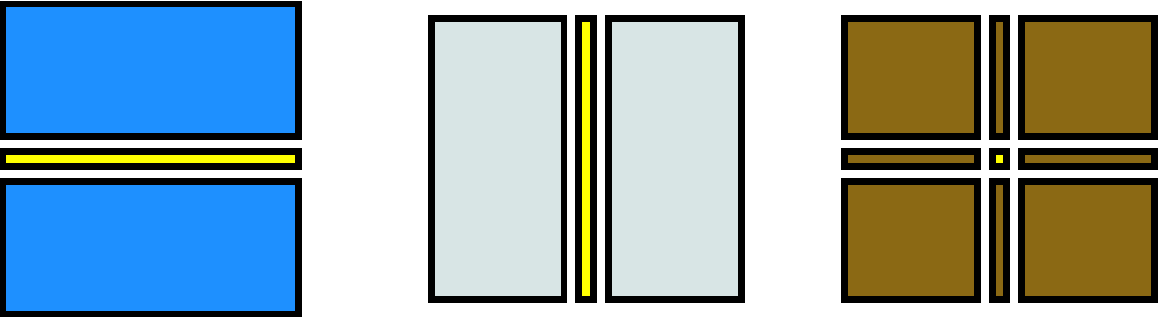
\includegraphics[scale=0.4]{UntiledMMIterationSpace.pdf}
\caption{Untiled Matrix Multiply Iteration Order}
\label{untiled_diagram}
\end{figure}

\begin{figure}
\centering
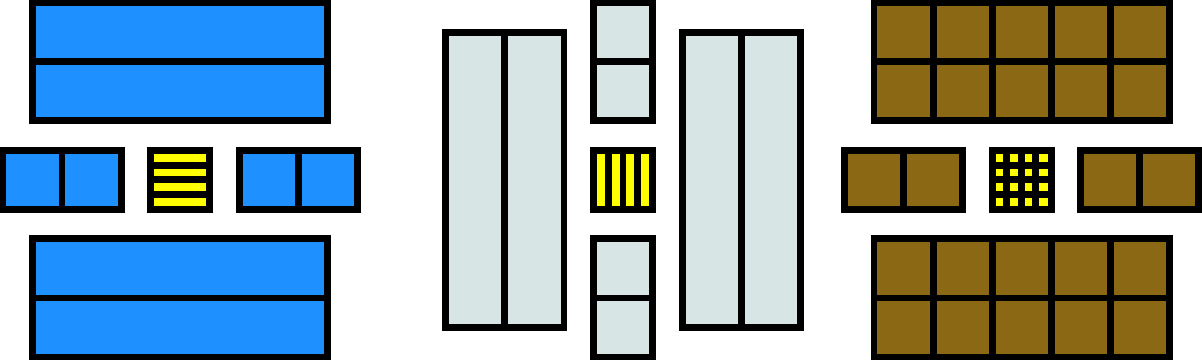
\includegraphics[scale=0.4]{TiledMMIterationSpace.pdf}
\caption{Tiled Matrix Multiply Iteration Order}
\label{tiled_diagram}
\end{figure}

\begin{lstlisting}[frame=single, label=tiledmm, caption={Tiled Matrix Multiply}, belowskip=0.5em]
for at in range(0, numRows, atSize):
  for bt in range(0, numCols, btSize):
    for i in range(at, at+atSize):
      for j in range(bt, bt+btSize):
        C[i,j] = 0
    for kt in range(0, rowLen, ktSize):
      for i in range(at, at+atSize):
        for j in range(bt, bt+btSize):
          for k in range(kt, kt+ktSize):
            C[i,j] += A[rowLen*i + k] * \
                      B[rowLen*j + k]
\end{lstlisting}

Cache tiling need not be for a single level of cache; tiling loops can be added for each level of cache in which to keep data resident between accesses.  In addition, tiling can be used to keep data resident in other levels of the memory hierarchy such as registers.

There has been much work on automating the process of tiling, including both generating the outer tiled loops from the inner ones as well as automating tile size selection given a tiled loop nest~\cite{Lam91, Wolf91} (REFS).  It might appear at first glance that determining good tile sizes for a given loop nest might be easy to do analytically.  Much work has been done on designing analytic models to estimate good tile sizes~\cite{Cole95, Shir12, Yoto03, Yoto05}.  However, while these models often perform fairly well, the state of the art for achieving the best performance is still offline autotuning to find the best settings for a particular target architecture, even for a problem as well-studied as matrix multiplication~\cite{Whal00}.

\section{Tiling Adverbs}
\label{tiling_transform}

In order to understand how our compiler automatically tiles Parakeet code, let us walk through matrix multiplication as an example.  In Listing \ref{parmm}, we see an implementation of matrix multipication.  This is a desugared version of the actual Parakeet code that we used in our benchmarks in Section \ref{evaluation}, and assumes that the second input matrix \lstinline{Y} has already been transposed for ease of presentation.

\begin{lstlisting}[label=parmm, caption={Parakeet Matrix Multiply}, belowskip=0.5em]
def dot(x, y):
  return Reduce(lambda x,y,acc: acc + x*y,
                x, y, init=0,
                combiner=lambda x,y: x+y)

def dgemm_1(x, Y):
  return Map(dot, Y, fixed=[x])
                
def dgemm(X, Y):
  return Map(dgemm_1, X, fixed=[Y])
\end{lstlisting}

Recall from the discussion in Section \ref{cache_tiling} that the \lstinline{AllPairs}pattern of data access in matrix multiplication involves temporal reuse such that cache tiling is very beneficial for performance.  At a high level, tiling an adverb (or loop) involves wrapping that adverb in another version of itself that breaks up its iteration pattern into smaller pieces.  The outer adverb iterates over tiles, while the inner one performs the original computation on the individual elements of each tile.

To support tiling in our compiler we introduce a set of \emph{tiled adverbs}, one for each existing adverb.  At a high level, the semantics of a tiled adverb are that it splits its inputs along some axis into tiles.  These tiles are then each consumed by executing the tiled adverb's nested function, and these partial results are combined in some structured way to form the final result.  Definitions of tiled adverbs' semantics are given in Figure \ref{def_tiled_adverbs}.  Note that our actual implementations of tiled adverbs are more efficient than these definitions might suggest.  The \lstinline{Split} operator in Figure \ref{def_tiled_adverbs} splits its arguments into tiles along the specified axis.  However, the actual tile sizes are left unspecified -- in the case of cache tiling until runtime, and in the case of register tiling until final compile time.
% 
% \begin{figure}
% \label{def_tiled_adverbs}
% \begin{lstlisting}[frame=none, backgroundcolor=\color{white}, belowskip=0.3em]
% def TiledMap(f, args, axis=0):
%   split_args = Split(args, axis)
%   partials = Map(f, split_args)
%   return Concatenate(partials)
% 
% def TiledReduce(f, args, combiner, init,
%                 axis=0):
%   split_args = Split(args, axis)
%   partials = Map(f, split_args)
%   return Reduce(combiner, partials,
%                 combiner, init)
% 
% def TiledScan(f, args, combiner, init,
%               axis=0):
%   split_args = Split(args, axis)
%   partials = Map(f, split_args)
%   concatenate last vals with init
%   scan this list
%   return the proper combination
% 
% def TiledAllPairs(f, X, Y, axis=0):
%   split_x = Split(X, axis)
%   split_y = Split(Y, axis)
%   partials = AllPairs(f, split_x, split_y)
%   return Concatenate(partials)
% \end{lstlisting}
% \caption{Tiled Adverb Definitions}
% \end{figure}

To see the problem with this, let's examine its cache behavior in detail.  Assume that we're tiling for L1 cache and that the matrices are much larger than the size of L1 cache so that even a single row from either matrix is on the order of the size of the cache (a realistic assumption for even medium sized data and current cache sizes).

First, the rows of the matrices \lstinline{X} and \lstinline{Y} are split into tiles.  Then, for every pair of tiles, every pair of rows from the tiles is passed to the function \lstinline{tiled_dot}.  At this point we can see that the \lstinline{TiledAllPairs} isn't going to do much to help cache behavior, as the single rows of the matrices are already large compared with the cache and so grouping them into even larger tiles is useless.

The next step of the computation involves splitting each pair of rows from \lstinline{X} and \lstinline{Y} into tiles, and then performing a dot product between each of these pieces.  Finally, these partial dot products are combined via addition to produce a final result.  In contrast with the \lstinline{TiledAllPairs}, the tiles from the \lstinline{TiledReduce} are able to benefit cache behavior, as they can be made small enough to fit into cache.  However, since they are splitting single rows of \lstinline{X} and \lstinline{Y}, the tiles' shapes are forced to be 1xN for some N.  It has been shown in various studies of tiling that the best tile shapes are typically closer to square, and ATLAS only considers square tiles in its search (REFS).  Regardless, we want the runtime's search to be able to find the best tile shapes and thus prefer not to restrict their shape in any way.

Thus we see that this straightforward approach to tiling the adverbs is problematic.  What we'd really prefer is for all of the tiling of every adverb to happen first, and then once the inputs are broken up into cache-friendly pieces only then to perform the inner computation.  A tiled version of matrix multiply that adheres to this principle is shown in Listing \ref{good_tiled_adverb_mm}.

\begin{lstlisting}[label=good_tiled_adverb_mm, caption={Good Tiled Matrix Multiply}, belowskip=0.5em]
def dot(x, y):
  return Reduce(lambda x,y,acc: acc + x*y,
                x, y, init=0,
                combiner=lambda x,y: x+y)

def dgemm(X, Y):
  return AllPairs(dot, X, Y)

def tiled_dot(X, Y):
  return TiledReduce(dgemm, X, Y,
                     init=0, axes=[1,1],
                     combiner=lambda x,y: x+y)

def tiled_dgemm_1(x, Y):
  return TiledMap(tiled_dot, Y, fixed=[x])
                     
def tiled_dgemm(X, Y):
  return TiledMap(tiled_dgemm_1, X, fixed=[Y])
\end{lstlisting}

The difference between this code and the last is that it's organized in the way we want: all of the tiling happens first, and the inner computation is performed on the cache-friendly pieces of the inputs. This solves both problems with the first version: the tiling of the \lstinline{TiledAllPairs} is now relevant in fitting the inner computation into cache, and all axes of the cache-relevant tiles' shapes are now free parameters that are settable at runtime.

While the transformation ``nest all tilings, then all original computation'' is legal in the case of matrix multiply, the case of general code is more complicated.  This is due to various factors such as the presence of additional non-adverb statements in functions which are tiled and control flow.  The full algorithm for our tiling transformation is given if Figure \ref{tiling_algorithm}.

\begin{figure*}[!t]
\centering
{\large
\begin{tabular}{| m{0.01cm}llm{13.8cm} |}
\hline
& & &\\
& function   & $::=$ & $\lambda x_1,\ldots,x_n.$statement$^+$\\
& statement  & $::=$ & $x$ \textbf{= } expression $|$ \textbf{return} expression\\
& expression & $::=$ & \textbf{map}($f$, $e_1,\ldots,e_n$) $|$ \textbf{reduce}($f$, $combiner, e_{init}, e_1,\ldots,e_n$) $|$ $e_1 \oplus e_2 $ $|$ $e_1[e_2]$ $|$ $x$\\
& & &\\
\hline
\end{tabular}
}
\caption{Simplified Parakeet Syntax}
\label{tiling_syntax}
\end{figure*}

\begin{figure*}
\centering
{\large
\begin{tabular}{| m{0.01cm}llm{14cm} |}
\hline
& & &\\
& $\llbracket\textbf{\textrm{return}}$ $e\rrbracket^{\alpha,\epsilon}_{stmt}$ & $::=$ & \textbf{return} $\llbracket e \rrbracket^{\alpha,\epsilon}_{expr}$\\
& & &\\
\hline
\end{tabular}
}
\caption{Tiling Transformation Algorithm}
\label{tiling_algorithm}
\end{figure*}

Before tiling an AST, we normalize every compound expression by breaking it up into a series of statements each of which only contains simple expressions.

\section{Parallelization and Online Tuning}
\label{online_tuning}

\section{Evaluation}
\label{evaluation}
Evaluate System on MM, K-Means, some Map-based Programs, Natural Join, and SVM, presenting overall performance improvements vs hand-tuned C and vs performance without any search and vs cherry-picked best parameter settings.

Make sure to present numbers on the exact overheads of recompilation and job reconfiguration.

Present exploration vs exploitation graphs.

\section{Related Work}
\label{related_work}
Our work builds upon a range of existing fields of study including just-in-time compilation, acceleration of high level array languages, loop optimizations, analytic performance modeling, and autotuning.

JIT compilation.

Python acceleration and the like (such as Numpy~\cite{Dubo96}, Numba, MaJIC~\cite{Alma02}, and Copperhead~\cite{Cata11}, as well as SciKit.learn~\cite{Pedr11}).

There has been extensive research on loop optimizations, including cache tiling, register tiling, data copying, data padding, and loop unrolling optimizations (e.g.~\cite{Lam91, Wolf91}). (Probably need a few more refs).  Our system builds on this body of work by providing a framework for automating optimization parameter selection, performing the search for good parameter settings online, and extending the applicability of these optimizations to unannotated, high-level code.

Analytic models for determining parameter settings for dense matrix multiplication~\cite{Cole95, Yoto03, Yoto05}.  Wolf et al.~developed an analytic model for use in a compiler to determine tiling and loop unrolling settings statically for sequential C and Fortran programs~\cite{Wolf96}.  Recent work on analytical bounds for optimal tile sizes~\cite{Shir12}.

The Ohio stuff on polyhedral models~\cite{Bond08}, including Pouchet's work on combining models with offline autotuning~\cite{Pouc10} and the paper on generating parameterized tiles~\cite{Hart09}.

PetaBricks~\cite{Anse09}.  Adaptic~\cite{Sama12}.

In recent years, offline autotuning has emerged as the accepted best practice for optimizing numerical code~\cite{Asan06}.  Libraries such as ATLAS for dense linear algebra~\cite{Whal00} and FFTW for Fourier transforms~\cite{Frig05} deliver the best performance available across a wide range of architectures and platforms for their specific problem domains via an extensive offline search performed at installation time.  Other recent work on offline autotuning includes that for stencil computations~\cite{Kami10,Datt08}.  While this technique is useful for either basic computational building blocks that are reused extensively (ATLAS and FFTW) or in the hands of expert programmers that are able to hand-program efficient low-level code with autotuning hooks inserted, our system expands the usefulness of autotuning to a broader audience and to rapid prototyping scenarios.

Chen et al. developed a system that automatically generates multiple candidate versions of C and Fortran programs by analyzing array references in loops and performing unroll-and-jam, cache tiling, copying, and TLB-oriented optimizations~\cite{Chen05b}.  Their focus is very much in the spirit of our work, but its offline search takes on the order of minutes and its algorithm for deriving parameterized code variants involves complex analysis of memory references and footprints.  We show that excellent performance is possible via a simple analytic model combined with efficient online search across parameter settings.

Active Harmony is a system for performing online autotuning that exposes a constraint specification language (CSL) for expressing tuning parameters~\cite{Tiwa11}.  The Active Harmony system doesn't address the problem of generating these tuning parameters, and its evaluation involved manual programming of the tuning parameters in the CSL as well as manual outlining of compute-intensive functions.  Active Harmony also targets loop-based programs written in C and Fortran.  Our system automatically inserts the necessary hooks for autotuning, and automatically extracts code sections from high level Python programs.  Thus we are able to improve performance of code written by non-expert programmers written in a high level language.  Finally, Active Harmony's recompilation is relatively heavy-weight and thus targets distributed clusters where it is possible to have dedicated code-generation servers.  In our system code generation is cheaper and is co-located with program execution on a single shared-memory node.

Tiwari et al.~presented a system that combines Active Harmony and Chen's system to auto-tune loop-based C and Fortran programs offline~\cite{Tiwa09}, thus targeting different use cases than does our system.

Knijnenburg et al.~presented a system for combining analytic models with offline autotuning to improve parameter settings of cache tiling and unrolling optimizations~\cite{Knij04}.  While they focus on two of the same optimizations as we do and use analytic models to improve their search, their search is performed offline and requires on the order of minutes to finish.

The ADAPT system~\cite{Voss99}.

Functional Skeleton stuff~\cite{Cole04, Darl95}.  DryadLINQ~\cite{Yu08, Yu09}.

Auto-vectorization~\cite{Kell12}.

\section{Conclusion}
\label{conclusion}
We have presented a system that automatically generates autotuning hooks in just-in-time compiled versions of code written in Parakeet+Python, a high-level numerical productivity language.  Our system automatically searches across different tuning parameter settings online, resulting in large performance improvements for a wide range of numerical programs.  We thus bring cutting-edge performance to non-expert programmers and to a rapid prototyping environment.

%\appendix
%\section{Appendix Title}

%This is the text of the appendix, if you need one.

%\acks

%Acknowledgments, if needed.

\bibliographystyle{abbrvnat}
\bibliography{../Parakeet}{}

% The bibliography should be embedded for final submission.

%\begin{thebibliography}{}
%\softraggedright

%\bibitem[Smith et~al.(2009)Smith, Jones]{smith02}
%P. Q. Smith, and X. Y. Jones. ...reference text...

%\end{thebibliography}

\end{document}
